\chapter{CG for Singular Systems}

We examine solving the equation Ax = \textbf{b} for a singular matrix A. The main obstacle in this problem is the matrix kernel, which is now a space of dimension one or larger (the kernel dimension of a regular matrix is zero, since the basis for a vector space consisting of only a zero vector is an empty set). Applying the CG algorithm on a starting vector which has non-zero components from the kernel of A can have unforeseen consequences on the convergence of the relative error.

For notation let us separate the vectors into two components - those from the span of A and those from the kernel of A. Let A be a square n x n singular matrix with a kernel of dimension m. Denoting \( \bold{v_1,v_2,... v_m} \in\) Span(A) such that \(\bold{\{v_1,...v_m\}}\) is the basis of Span(A) and \( \bold{w_{m+1},w_{m+2},... w_n} \in\) Ker(A) such that \(\bold{\{w_{m+1},w_{m+2},... w_n\}}\) is the basis of Ker(A), and \(a_i, b_i\) are real coefficients,  then
\begin{equation}\label{b}
 \bold{b} = \sum_{i=1}^m{a_i \bold{v_i}} + \sum_{i=m+1}^n{b_i \bold{w_i}} = \bold{b^s + b^{\perp}}.
\end{equation}
I will split all other vectors the same way, e.g. \(\bold{r = r^s + r^{\perp}} \),...


Since we wish to measure the convergence rate using the so-called energy norm, it has to be redefined on the new space, because the presence of the matrix kernel (with dimension larger or equal to 1) causes our original definition to lose the characteristic of positive definiteness. 
From here on the energy norm will thus be redefined as \(\boldsymbol{\|x\|_{{A}} = \sqrt{(x,x)_{A}}}\)    \(\forall{x} \in\)  Span(A).

\section{Consistent Systems}

Let us consider vector \(\bold{b} \in\) Span(A). This means \(\bold{b^{\perp} = 0}\), thus 
\begin{equation}   
\bold{b} = \sum_{i=1}^m{a_i \bold{v_i}} = \bold{b^s}
\end{equation} 
where \(\{a_k\}_{i=1}^m\) are real coefficients and \(\bold{\{v_1,...v_m\}}\) is the basis of Span(A).
Using this as input for the CG algorithm gives the following result:
\begin{algorithm}
\caption{Conjugate Gradient Algorithm for Systems with \(\bold{b} \in\) Span(A)}
\begin{algorithmic}[1]
    \STATE \textbf{Input:} $A$, $\boldsymbol{b}$, $x_0$
    \STATE $r_0 := \boldsymbol{b} - Ax_0 = \boldsymbol{b^s} - Ax_0$
    \STATE $p_0 := r_0 = r_0^s$
    \FOR{$k = 1, 2, \ldots$}
        \STATE $\gamma_{k-1} := \frac{r_{k-1}^T r_{k-1}}{p_{k-1}^T A p_{k-1}} =  \frac{(r_{k-1}^s)^T r_{k-1}^s}{(p_{k-1}^s)^T A p_{k-1}^s}$
        \STATE $x_k := x_{k-1} + \gamma_{k-1} p_{k-1} = x_{k-1} + \gamma_{k-1} p_{k-1}^s$
        \STATE $r_k := r_{k-1} - \gamma_{k-1} A p_{k-1} = x_{k-1} + \gamma_{k-1} p_{k-1}^s$
        \STATE $\delta_k := \frac{r_k^T r_k}{r_{k-1}^T r_{k-1}} = \frac{(r_k^s)^T r_k^s}{(r_{k-1}^s)^T r_{k-1}^s}$
        \STATE $p_k := r_k + \delta_k p_{k-1} = r_k^s + \delta_k p_{k-1}^s$
    \ENDFOR
\end{algorithmic}
\end{algorithm}



    Given \(x_{k-1},\,r_{k-1},\,p_{k-1} \in\) Span(A), it can be observed that the vectors generated in the following iteration \( x_k,\,r_k \) and \(p_k \) stay in the Span(A) as well. We could say the algorithm "doesn't notice" the Kernel space of A unless we pick \(x_0\) such, that it's component lies in Ker(A). Since we set \(x_0 = 0\), \(r_0 = \boldsymbol{b_s} - Ax_0\) and \(p_0 := r_0\), we now know that the solution \(x_k\) will always belong to Span(A) and the CG method will converge to the minimum norm solution of, since the (preconditioned, \cite{Kaasschieter}) CG algorithm applied on the equation \(Ax = \bold{b}^s\) generates a sequence of approximations \(x_1,\, x_2,... \) such that for i = 1, 2, ... it holds that \(x_i \in \mathcal{K}_i(A,r_0)\) and \(\mathcal{K}_i \subset Span(A)\).

   %% This solution can be viewed as a least-squares approximation of the solution of \(Ax = \bold{b}\) for all vectors \(\bold{b}\) such that their orthogonal projection onto Span(A) is equal to \(\bold{b}^s\).

\section{Non-convergent Case}

The worst-case scenario is having the right-hand side vector \(\bold{b}\) completely in the kernel of the matrix A. Setting \(\bold{b = b^\perp}\), meaning that 
\begin{equation}
    \bold{b} = \sum_{i=m+1}^n{b_i \bold{w_i}} = \bold{b^\perp}
\end{equation}
where \(\{b_i\}\) are real coefficients and \(\bold{\{w_{m+1},...w_n\}}\) is the basis of Ker(A), let us look at the effect this has on the CG algorithm.

In the first iteration of the algorithm (with the input A, \textbf{b} and \(x_0\)), the value of \(\gamma\) will have the form:

\begin{itemize}
    \item \(r_0 := \bold{b} - Ax_0 = \boldsymbol{b^\perp} - Ax_0\)
    \item \(p_0 := r_0\)
    \item \(\gamma_{0} := \frac{r_{0}^Tr_{0}}{p_{0}^TAp_{0}}\)
\end{itemize}

However, substituting into the expression of \(\gamma_{0}\) gives: \begin{equation}
    p_{0}^TAp_{0} = r_{0}^TAr_{0} = (\boldsymbol{b^\perp} - Ax_0)^TA(\boldsymbol{b^\perp} - Ax_0) = x_0A^3x_0.
\end{equation}
    The value of gamma is thus heavily reliant on the value of \(x_0\), which is set as 0 in our computations unless a specific problem offers a better starting approximation. For this value the algorithm collapses, as the value of gamma reaches \(\infty\) in the first iteration and convergence becomes impossible.

\section{Perturbed Systems}

Having explored both extreme cases for the right-hand side vector b, it remains to look at the general case of \(\bold{b = \bold{b^s} + \bold{b^\perp}} \) such that \(\bold{b^s} \neq 0, \bold{b^\perp} \neq 0\). In other words, at least one coefficient \(a_i\) and at least one coefficient \(b_i\) is non-zero in \eqref{b}.

To analyze the convergence of the CG method applied on the equation \(Ax = \bold{b}\), such that \(A\) is a singular, symmetrical, positive semi-definite matrix, I will deconstruct the algorithm into the range space and the kernel space of matrix A, as it was done in \cite{Hayami08}. 
I shall do this for a general starting approximation \(\bold{x_0 = x_0^s + x_0^\perp}\), and later on simplify for the popular choice \(x_0 = 0\).

\begin{algorithm}
\caption{Modified Conjugate Gradient Algorithm}
\label{alg:modified_cg}
\begin{algorithmic}[1]
  \STATE \textbf{Input:} Positive definite matrix $A$, vectors $\boldsymbol{b}^s$, $\boldsymbol{b}^\perp$, initial guess $x_0 = x_0^s + x_0^\perp$
  \STATE $r_0^s := \boldsymbol{b}^s - A x_0^s$
  \hfill $r_0^{\perp} := b^{\perp}$
  \STATE $p_0^s := r_0^s$
  \hfill $p_0^{\perp} := r_0^{\perp}$
  \FOR{$k = 1, 2, \ldots$}
    \STATE $\gamma_{k-1} = \frac{(r_{k-1}^s)^T r_{k-1}^s + (\boldsymbol{b}^\perp)^T \boldsymbol{b}^\perp}{(p_{k-1}^s)^T A p_{k-1}^s}$
    \STATE $x_k^s := x_{k-1}^s + \gamma_{k-1} p_{k-1}^s$ \hfill $x_k^{\perp} := x_{k-1}^{\perp} + \gamma_{k-1} p_{k-1}^{\perp}$
    \STATE $r_k^s := r_{k-1}^s - \gamma_{k-1} A p_{k-1}^s$
    \hfill $r_k^{\perp} := b^{\perp}$
    \STATE $\delta_k = \frac{(r_k^s)^T r_k^s + (\boldsymbol{b}^\perp)^T \boldsymbol{b}^\perp}{(r_{k-1}^s)^T r_{k-1}^s + (\boldsymbol{b}^\perp)^T \boldsymbol{b}^\perp}$
    \STATE $p_k^s := r_k^s + \delta_k p_{k-1}^s$
    \hfill $p_k^{\perp} := b^{\perp} + \delta_k p_{k-1}^{\perp}$
  \ENDFOR
\end{algorithmic}
\end{algorithm}


The starting vectors in the kernel space of A don't contain any component of \(\bold{x_0^\perp}\). This component appears only in the computation of \(x_k^\perp\).
The value of the residual vector component in the kernel space \(r_k^\perp\) is constant through every iteration. \(\gamma\) contains an additional value of \(\frac{ (b^{\perp})^T b^{\perp}}{(p_{k-1}^s)^T A p_{k-1}^s}\) only in the numerator, whereas \(\delta\) has the addition of \((b^\perp)^Tb^\perp\) in the numerator as well as in the denominator.

Our focus is on the behaviour of the vectors \(x_k^\perp \text{ and } r_k^\perp\) throughout the run-time of our algorithm. How quickly do they grow (with respect to the A-norm?) and how much do they interfere with convergence?
To answer these questions, it might be useful to decompose the vectors into constants and the respective starting vectors.
\begin{equation}
\begin{aligned}
x_k^\perp &= x_{k-1}^\perp + \gamma_{k-1}p_{k-1}^\perp \\
&= x_{k-2}^\perp + \gamma_{k-2}p_{k-2}^\perp  + \gamma_{k-1}p_{k-1}^\perp\\
&= \gamma_{k-1}p_{k-1}^\perp + \gamma_{k-2}p_{k-2}^\perp  + \gamma_{k-3}p_{k-3}^\perp   \\
&\hphantom{=} \cdots  \\ 
&\quad + \gamma_{0}p_{0}^\perp + x_0^\perp  \\
&=\Pi_{i=0}^{k-1}\gamma_{i}p_{i}^\perp + x_0^\perp. \\
x_k^\perp &= \Pi_{i=0}^{k-1}\gamma_{i}p_{i}^\perp \indent\text{for \(x_0^\perp = 0\).}
\label{x_k decomp}
\end{aligned}
\end{equation}

The component \(x_0^\perp\) is constant throughout the runtime of the algorithm. The component \(\Pi_{i=0}^{k-1}\gamma_{i}p_{i}^\perp \) must be responsible for the divergence of the relative error \(\frac{x_k - x_0}{\|x_k - x_0\|_A}\).

To understand how quickly this component grows, we will do the same analysis on \(p_k^\perp\).

\begin{equation}
\begin{aligned}
p_k^\perp &= b^\perp + \delta_kp_{k-1}^\perp \\
&= b^\perp + \delta_kb^\perp + \delta_k\delta_{k-1}p_{k-2}^\perp \\
&\hphantom{=} \cdots \\
&\quad + \delta_k\delta_{k-1} \cdots \delta_{k-i} b^\perp + \dots + (\Pi_{i=0}^{k-1}\delta_{k-i})p_0^\perp.
\end{aligned}
\label{p_k decomp}
\end{equation}
Which can be simplified using the knowledge that \(p_0^\perp = b^\perp\) and 
\begin{equation}
\begin{aligned}
\delta_k\delta_{k-1} &= \frac{(r_k^s)^T r_k^s + (b^\perp)^T b^\perp}{(r_{k-1}^s)^T r_{k-1}^s + (b^\perp)^T b^\perp} 
\cdot \frac{(r_{k-1}^s)^T r_{k-1}^s + (b^\perp)^T b^\perp}{(r_{k-2}^s)^T r_{k-2}^s + (b^\perp)^T b^\perp} \\
&= \frac{(r_k^s)^T r_k^s + (b^\perp)^T b^\perp}{(r_{k-2}^s)^T r_{k-2}^s + (b^\perp)^T b^\perp}.
\end{aligned}
\label{delta_k_decomp}
\end{equation}
We get
\begin{equation}
\begin{aligned}
p_k^\perp &= b^\perp + \delta_kp_{k-1}^\perp \\
&= b^\perp (1 + \delta_k \sum_{i=1}^{k-1} \frac{1}{(r_{k-i}^s)^T r_{k-i}^s + (b^\perp)^T b^\perp}) \\
&\hphantom{=} + \frac{(r_k^s)^T r_k^s + (b^\perp)^T b^\perp}{(r_{0}^s)^T r_{0}^s + (b^\perp)^T b^\perp} b^\perp \\
&= b^\perp (1 + [(r_k^s)^T r_k^s + (b^\perp)^T b^\perp] \sum_{i=0}^{k-1} \frac{1}{(r_{i}^s)^T r_{i}^s + (b^\perp)^T b^\perp}).
\end{aligned}
\label{p_k_full}
\end{equation}
And after connecting the results
\begin{equation}
    \begin{aligned}
        x_k^\perp &= \Pi_{i=0}^{k-1}\gamma_{i}p_{i}^\perp\\
        &= \Pi_{i=0}^{k-1}\gamma_{i}b^\perp (1 + [(r_i^s)^T r_i^s + (b^\perp)^T b^\perp] \sum_{j=0}^{i-1} \frac{1}{(r_{j}^s)^T r_{j}^s + (b^\perp)^T b^\perp}).
    \end{aligned}
\end{equation}

We can see that the component of \(x_k\) which lies in the kernel of matrix A is not easy to analyze analytically. It is an obscure equation, that we will further analyze experimentally.

\subsection{Experimental analysis}

We will first consider a matrix called the "Strakoš matrix" (used by Zdeněk Strakoš, who is known for his work on Krylov subspace methods). It is reliant on a parameter \(\rho \in {(0,1]}\), which influences the distribution of eigenvalues over a given interval [a,b]. We will set these values along with the size of the matrix N, and construct the eigenvalues in the following way

\[\lambda_1 = a \]
\[\lambda_N = b \]
\begin{equation}
    \lambda_i = \lambda_1 + \frac{i-1}{N-1}*(b-a)*\rho^{(n-i+1)}
\end{equation}

\begin{figure}[htp]
\centering
\title{Eigenvalue distribution}
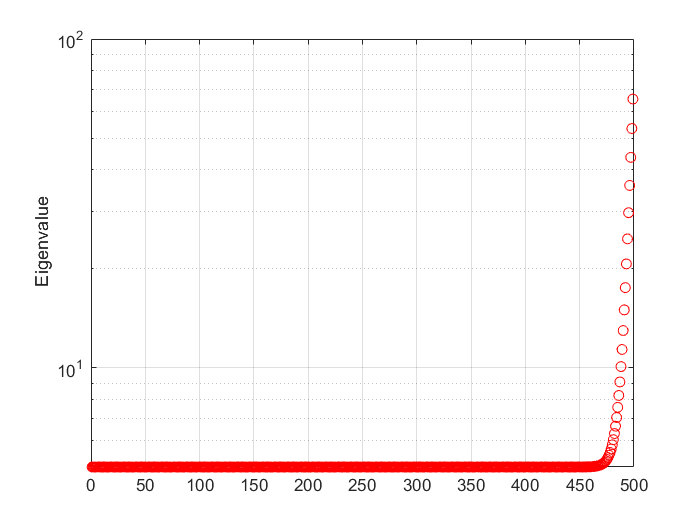
\includegraphics[width=0.7\linewidth]{img/diagonal_val.png}
\caption{Eigenvalues of the Strakoš matrix with dimensions N = 500, [a, b] = [5, 100], \(\rho = 0.8\)}. 
\label{fig:eig distribution}
\end{figure}
 
Using this set of eigenvalues, a singular, symmetrical positive semi-definite matrix of dimension N+1 is constructed, with dimension of the kernel equal to one (this dimension is chosen for simplicity). 
(The use of the Strakoš matrix gives the opportunity to test out different eigenvalue distributions, investigate rounding errors stemming from clustered eigenvalues, and explore small perturbations in almost-singular matrices.)


Next, a right-hand side vector b is generated and then perturbed using a random normed vector from the kernel space that is scaled by a parameter \(\delta = {0, 1e^{-6},  1e^{-4}, 1e^{-2}}\). We then apply the CG method to solve \(A\bold{x}=\bold{b}\) with the starting vector \(\bold{x_0 = 0}\). 

\begin{figure}[ht]
\centering
\title{Relative error}
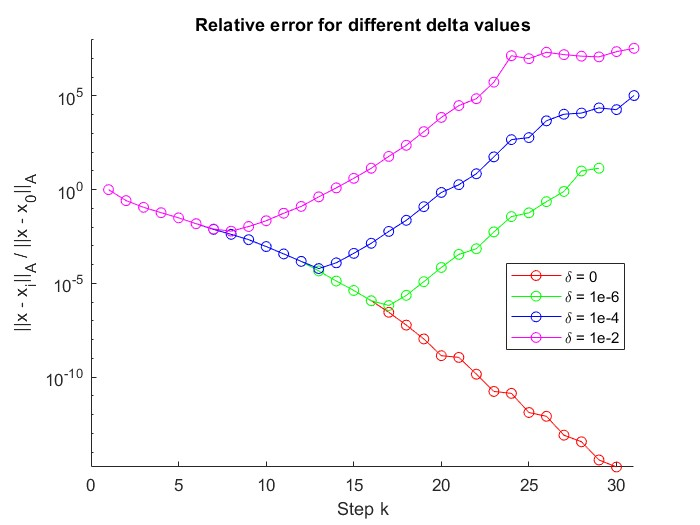
\includegraphics[width=\linewidth]{img/relative_error_different_delta_val.jpg}
\caption{Comparison of relative error in each step k of the CG method for different delta values. Matrix dimensions N = 500, \(\rho = 0.8\) Inspired by  \cite{Hayami08}}. 
\label{fig:relative error}
\end{figure}


\begin{figure}[htp]
    \centering
    \begin{minipage}{0.48\textwidth}
        \centering
        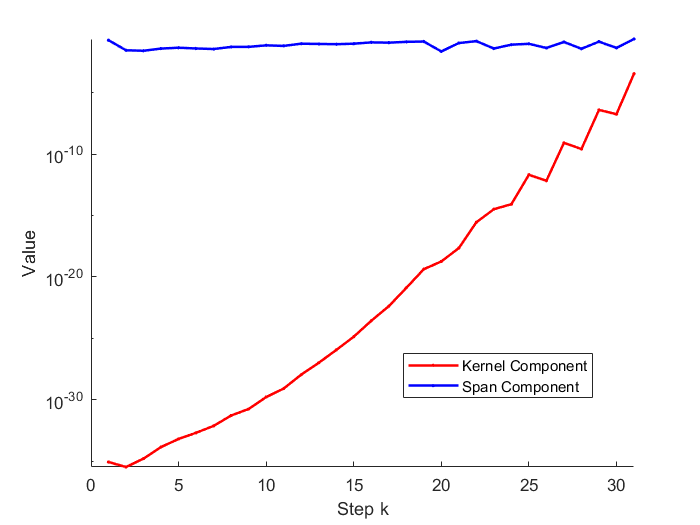
\includegraphics[width=\linewidth]{img/gamma1comp.png}
        \caption{\(\delta = 0\)}
    \end{minipage}
    \hfill
    \begin{minipage}{0.48\textwidth}
        \centering
        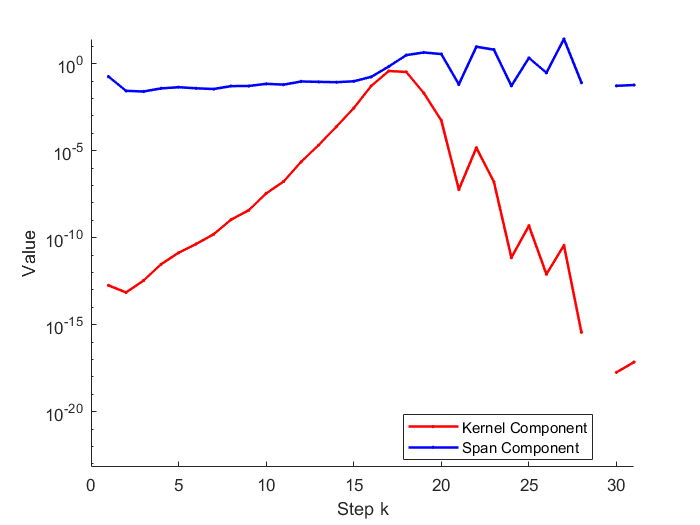
\includegraphics[width=\linewidth]{img/gamma2comp.png}
        \caption{\(\delta = 1e^{-6}\)}
    \end{minipage}
    \vfill
    \begin{minipage}{0.48\textwidth}
        \centering
        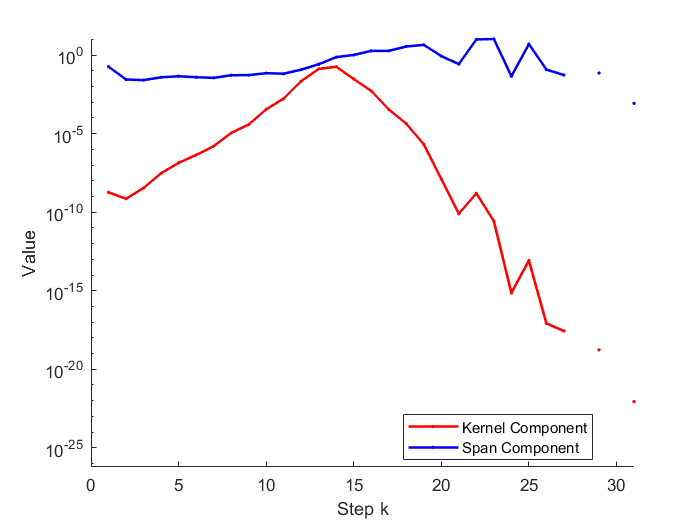
\includegraphics[width=\linewidth]{img/gamma3comp.png}
        \caption{\(\delta = 1e^{-4}\)}
    \end{minipage}
    \hfill
    \begin{minipage}{0.48\textwidth}
        \centering
        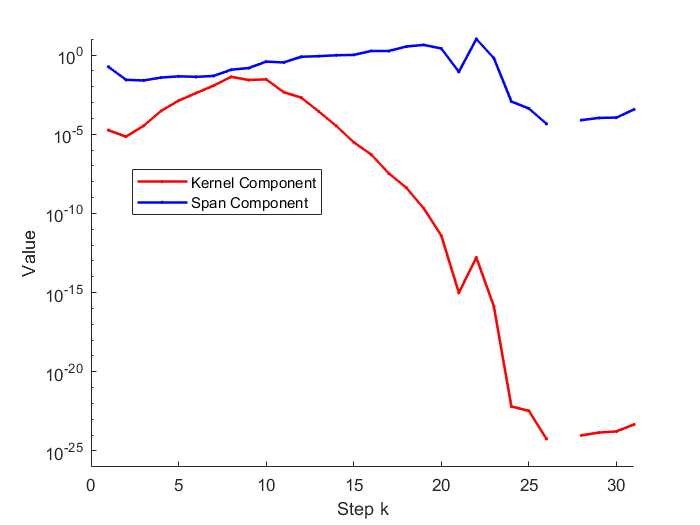
\includegraphics[width=\linewidth]{img/gamma4comp.png}
        \caption{\(\delta = 1e^{-2}\)}
    \end{minipage}
    \caption{Seperating \(\gamma\) into its span and kernel subspaces, we can notice their relative values (in the norm).}
    \label{fig:fig4}
\end{figure}